\documentclass[11pt,letterpaper]{article}
\usepackage[T1]{fontenc}
\usepackage[scaled]{helvet}
\renewcommand{\familydefault}{\sfdefault}
\usepackage{amsmath,amssymb}
\usepackage[margin=0.8in,bottom=0.9in]{geometry}
\usepackage[most]{tcolorbox}
\usepackage{tikz}
\usetikzlibrary{calc}
\usepackage{enumitem}
\usepackage{array}
\usepackage{needspace}
\usepackage{fancyhdr}
\usepackage{pifont}

% ---- Palette "F. Bright & Playful" ----
\definecolor{fmtitle}{HTML}{3D2C8D}
\definecolor{fmkey}{HTML}{0096C7}
\definecolor{fmwatch}{HTML}{2BB673}
\definecolor{fmturn}{HTML}{F4A100}
\definecolor{fmmistake}{HTML}{EF476F}
\definecolor{fmnotice}{HTML}{9B5DE5}
\definecolor{fmgray}{HTML}{6B6B6B}

\pagestyle{fancy}
\fancyhf{}
\renewcommand{\headrulewidth}{0pt}
\fancyfoot[C]{\footnotesize\color{fmgray}\textcopyright\ 2026 FangMath. All rights reserved.}
\fancyfoot[R]{\footnotesize\color{fmgray}\thepage}
\setlength{\parindent}{0pt}
\setlength{\parskip}{3pt}

\newcommand{\badge}[1]{\colorbox{fmtitle}{\color{white}\bfseries\small\ #1\ }}
\newcommand{\leveltag}[2]{\colorbox{#1}{\color{white}\bfseries\scriptsize\ #2\ }}
\newcommand{\LE}{\leveltag{fmwatch}{EASY}}
\newcommand{\LM}{\leveltag{fmturn}{MEDIUM}}
\newcommand{\LH}{\leveltag{fmmistake}{HARD}}

\newcommand{\sectionbar}[2]{\needspace{6cm}\par\vspace{4mm}
  \begin{tcolorbox}[enhanced,colback=fmtitle,colframe=fmtitle,arc=2mm,
    left=4mm,top=1.5mm,bottom=1.5mm]
  \color{white}\bfseries\large #1\hfill{\normalsize\mdseries #2}
  \end{tcolorbox}}

\newtcolorbox{keyidea}{enhanced,breakable,colback=white,colframe=fmkey,boxrule=1pt,arc=2mm,
  title={Key Idea},coltitle=fmkey,fonttitle=\bfseries,
  attach boxed title to top left={xshift=4mm,yshift=-2mm},
  boxed title style={colback=white,colframe=fmkey,boxrule=0.9pt}}
\newtcolorbox{watchme}{enhanced,colback=white,colframe=fmwatch,boxrule=1pt,arc=2mm,
  title={Watch Me --- Worked Example},coltitle=fmwatch,fonttitle=\bfseries,
  attach boxed title to top left={xshift=4mm,yshift=-2mm},
  boxed title style={colback=white,colframe=fmwatch,boxrule=0.9pt}}
\newtcolorbox{mistakebox}{enhanced,breakable,colback=white,colframe=fmmistake,boxrule=1pt,arc=2mm,
  title={Common Mistake},coltitle=fmmistake,fonttitle=\bfseries,
  attach boxed title to top left={xshift=4mm,yshift=-2mm},
  boxed title style={colback=white,colframe=fmmistake,boxrule=0.9pt}}
\newtcolorbox{yourturn}{enhanced,breakable,colback=white,colframe=fmturn,boxrule=1pt,arc=2mm,
  title={Your Turn},coltitle=fmturn,fonttitle=\bfseries,
  attach boxed title to top left={xshift=4mm,yshift=-2mm},
  boxed title style={colback=white,colframe=fmturn,boxrule=0.9pt}}
\newtcolorbox{answerbox}[1]{enhanced,breakable,colback=white,colframe=fmwatch,boxrule=1pt,arc=2mm,
  title={#1},coltitle=fmwatch,fonttitle=\bfseries,
  attach boxed title to top left={xshift=4mm,yshift=-2mm},
  boxed title style={colback=white,colframe=fmwatch,boxrule=0.9pt}}

\newcommand{\work}[1]{\par\vspace{#1}}
\setlist[enumerate]{itemsep=2pt,topsep=3pt}

% ---------------- extra boxes ----------------
\newtcolorbox{notebox}{enhanced,breakable,colback=white,colframe=fmnotice,boxrule=1pt,arc=2mm,
  title={Notice},coltitle=fmnotice,fonttitle=\bfseries,
  attach boxed title to top left={xshift=4mm,yshift=-2mm},
  boxed title style={colback=white,colframe=fmnotice,boxrule=0.9pt}}
\newtcolorbox{exbox}{enhanced,colback=white,colframe=fmwatch,boxrule=0.8pt,arc=2mm,
  title={Example},coltitle=fmwatch,fonttitle=\bfseries\small,
  attach boxed title to top left={xshift=4mm,yshift=-2mm},
  boxed title style={colback=white,colframe=fmwatch,boxrule=0.8pt},fontupper=\small}
\newcommand{\topicbar}[1]{\needspace{4.5cm}\par\vspace{5mm}
  \begin{tcolorbox}[enhanced,colback=fmtitle,colframe=fmtitle,arc=2mm,left=4mm,top=1.5mm,bottom=1.5mm]
  \color{white}\bfseries\large #1
  \end{tcolorbox}}
\usepackage{multicol}

% ---------------- practice layout ----------------
\newcommand{\workline}{\par\vspace{7mm}{\color{gray!55}\rule{\linewidth}{0.4pt}}}
\newcommand{\worklines}[1]{\foreach \i in {1,...,#1}{\workline}}
\newcommand{\prob}[3]{\needspace{#3}\par\vspace{3mm}{\color{fmturn}\bfseries #1.}\ #2\par}
\newcommand{\ansline}{\par\vspace{4mm}\hfill\textbf{Answer:}\ \rule{5cm}{0.4pt}\par}
\newcommand{\keyitem}[3]{\needspace{3.2cm}\par\vspace{2mm}
  \begin{tcolorbox}[enhanced,colback=white,colframe=fmwatch!60,boxrule=0.6pt,arc=1.5mm,left=3mm,top=1.5mm,bottom=1.5mm]
  {\color{fmwatch}\bfseries #1.}\quad\small #2\par\vspace{1mm}
  \normalsize\textbf{Answer: #3}
  \end{tcolorbox}}


\usetikzlibrary{arrows.meta}
\providecommand{\iskey}{0}
% fill-in blank: line for students, pink answer in the key
\newcommand{\fb}[2][2.6cm]{\ifnum\iskey=1 \underline{\makebox[#1][c]{\color{fmmistake}\bfseries #2}}\else\underline{\makebox[#1]{}}\fi}
% answer line for practice problems
\newcommand{\pans}[2][3.2cm]{\ifnum\iskey=1 \underline{\makebox[#1][c]{\color{fmmistake}\bfseries #2}}\else\rule{#1}{0.4pt}\fi}
\newcommand{\vid}[1]{{\color{fmgray}\small\textit{\ding{43} Video: #1}}}
\newcommand{\pt}[2]{\fill (#1) circle (2.2pt) node[above=1pt,font=\small]{$#2$};}

\usetikzlibrary{decorations.pathreplacing}
% three points on a segment with lengths written above the pieces: #1,#2,#3 letters; #4,#5 piece labels; #6 whole label (below)
\newcommand{\threept}[6]{\begin{tikzpicture}[x=1cm]\draw[thick] (0,0)--(3.6,0);
\fill (0,0) circle(2.2pt) node[below=2pt,font=\small]{$#1$} (1.4,0) circle(2.2pt) node[below=2pt,font=\small]{$#2$} (3.6,0) circle(2.2pt) node[below=2pt,font=\small]{$#3$};
\node[above,font=\small] at (0.7,0.02){#4};\node[above,font=\small] at (2.5,0.02){#5};
\if\relax\detokenize{#6}\relax\else\draw[gray,decorate,decoration={brace,amplitude=4pt,mirror}] (0,-0.45)--(3.6,-0.45) node[midway,below=4pt,font=\small]{#6};\fi
\end{tikzpicture}}
\newcommand{\sdp}[3]{\begin{minipage}[t][2.4cm]{0.48\linewidth}{\color{fmturn}\bfseries #1.}\ #2\par\vfill\hfill \pans[3.6cm]{#3}\end{minipage}}
\newcommand{\figp}[4]{\begin{minipage}[t]{0.48\linewidth}{\color{fmturn}\bfseries #1.}\ #2\par\vspace{1mm}\centering #3\par\vspace{2mm}\raggedleft \pans[2.6cm]{#4}\end{minipage}}
\newcommand{\algp}[3]{\begin{minipage}[t][4.6cm]{0.48\linewidth}{\color{fmturn}\bfseries #1.}\ #2\par\vfill\hfill \pans[4.2cm]{#3}\end{minipage}}


% ch2: long key answers wrap inside their column instead of running into the next one
\newlength{\pw}
\renewcommand{\pans}[2][3.2cm]{\ifnum\iskey=1 \settowidth{\pw}{\bfseries #2}\ifdim\pw>#1 \parbox[b]{#1}{\raggedleft\color{fmmistake}\bfseries\small #2}\else\underline{\makebox[#1][c]{\color{fmmistake}\bfseries #2}}\fi\else\rule{#1}{0.4pt}\fi}
\begin{document}
\ifnum\iskey=1 \colorbox{fmwatch}{\color{white}\bfseries\small\ ANSWER KEY\ }\else\badge{PRACTICE}\fi\hfill{\small\color{fmgray}Geometry \textperiodcentered\ Lesson 2.3}\par\vspace{4mm}
{\color{fmtitle}\LARGE\bfseries Postulates \& Diagrams --- Practice\ifnum\iskey=1 \ --- Answer Key\fi}\par\vspace{1mm}
{\color{fmgray}A worked example comes before each type. Show your thinking.}\par\vspace{3mm}
Name: \rule{6cm}{0.4pt}\hspace{1cm}Date: \rule{3.5cm}{0.4pt}\par\vspace{2mm}

\needspace{6cm}\topicbar{Type 1 \quad Which Postulate?}
\begin{watchme}``Points $P$ and $Q$ lie in plane $M$, so line $PQ$ lies in plane $M$.''\par
Postulate: if two points lie in a plane, then the \textbf{line containing them} lies in that plane.\par
\textbf{Other postulates:} two points $\to$ one line; three noncollinear points $\to$ one plane; two lines meet in one point; two planes meet in one line.\end{watchme}
\needspace{3.4cm}\noindent\sdp{1}{How many lines pass through points $A$ and $B$?}{exactly one}\hfill\sdp{2}{How many planes contain three noncollinear points $J$, $K$, $L$?}{exactly one}\par\vspace{2mm}
\needspace{3.4cm}\noindent\sdp{3}{Two different planes intersect. What is their intersection?}{a line}\hfill\sdp{4}{Two different lines intersect. What is their intersection?}{a point}\par

\needspace{7cm}\topicbar{Type 2 \quad What Can You Assume From a Diagram?}
\begin{watchme}\begin{minipage}[c]{0.34\linewidth}\centering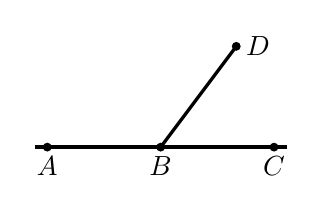
\begin{tikzpicture}[scale=0.8]\draw[very thick] (-2,0)--(2,0); \draw[very thick] (0,0)--(1.2,1.6); \fill (-1.8,0) circle(2pt) node[below]{$A$} (1.8,0) circle(2pt) node[below]{$C$} (0,0) circle(2pt) node[below]{$B$} (1.2,1.6) circle(2pt) node[right]{$D$};\end{tikzpicture}\end{minipage}\hfill
\begin{minipage}[c]{0.62\linewidth}\textbf{Yes:} $A$, $B$, $C$ are collinear; $\angle ABD$ and $\angle DBC$ are a linear pair (drawn).\par
\textbf{No:} $\angle DBC = 60^\circ$, or $AB = BC$ --- no marks say so.\end{minipage}\end{watchme}
\needspace{4.2cm}\noindent\begin{minipage}[t]{0.42\linewidth}\centering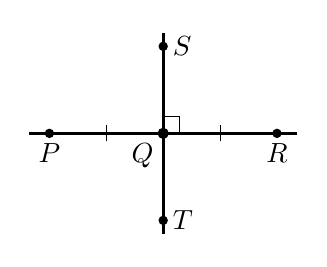
\begin{tikzpicture}[scale=0.85]\draw[very thick] (-2,0)--(2,0); \draw[very thick] (0,-1.5)--(0,1.5); \draw (0,0)--(0.25,0)--(0.25,0.25)--(0,0.25); \fill (-1.7,0) circle(2pt) node[below]{$P$} (1.7,0) circle(2pt) node[below]{$R$} (0,1.3) circle(2pt) node[right]{$S$} (0,-1.3) circle(2pt) node[right]{$T$}; \fill (0,0) circle(2.4pt) node[below left]{$Q$}; \draw (-0.85,-0.12)--(-0.85,0.12) (0.85,-0.12)--(0.85,0.12);\end{tikzpicture}\end{minipage}\hfill
\begin{minipage}[t]{0.55\linewidth}Use the diagram. Write \textbf{yes} or \textbf{no}.\par\vspace{1mm}
{\color{fmturn}\bfseries 5.} $P$, $Q$, $R$ are collinear. \hfill\pans[1.6cm]{yes}\par\vspace{2mm}
{\color{fmturn}\bfseries 6.} $\overline{PR} \perp \overline{ST}$. \hfill\pans[1.6cm]{yes}\par\vspace{2mm}
{\color{fmturn}\bfseries 7.} $PQ = QR$. \hfill\pans[1.6cm]{yes}\par\vspace{2mm}
{\color{fmturn}\bfseries 8.} $SQ = QT$. \hfill\pans[1.6cm]{no}\end{minipage}\par

\needspace{6cm}\topicbar{Type 3 \quad Sketch It}
\begin{watchme}``Sketch two planes that intersect in line $\ell$.'' Draw two flat sheets crossing each other and label the crossing line $\ell$.\par
Tip: use tick marks and right-angle marks only for things that are given.\end{watchme}
\needspace{4.6cm}\noindent\algp{9}{Sketch line $m$ intersecting plane $X$ at point $A$.}{a line piercing the plane at $A$}\hfill\algp{10}{Sketch $\overline{AB}$ with midpoint $M$ (use tick marks).}{$AM$ and $MB$ each with one tick}\par

\needspace{6cm}\topicbar{Type 4 \quad Always, Sometimes or Never?}
\begin{watchme}``Three points are coplanar.'' \quad Through any three points there is at least one plane. \quad \textbf{Answer: always.}\par
``Three points are collinear.'' \quad Some are on one line, some are not. \quad \textbf{Answer: sometimes.}\end{watchme}
\needspace{3.4cm}\noindent\sdp{11}{Two points are collinear.}{always}\hfill\sdp{12}{Two lines intersect in two points.}{never}\par\vspace{2mm}
\needspace{3.4cm}\noindent\sdp{13}{Four points are coplanar.}{sometimes}\hfill\sdp{14}{Two planes intersect in a point only.}{never}\par\vspace{2mm}
\needspace{3.4cm}\noindent\sdp{15}{A line and a plane intersect in one point.}{sometimes}\hfill\sdp{16}{\LH\ Through a line and a point not on it, how many planes pass?}{exactly one}\par
\end{document}
